% ============================================================
%  CHAPTER 2: LITERATURE REVIEW
% ============================================================

\chapter{LITERATURE REVIEW}
\label{chap:literature_review}

\section{Virtual Private Networks and Tunneling Principles}
\label{sec:vpn_tunneling_principles}

The theoretical and architectural foundations of Virtual Private Networks (VPNs) originate in the necessity to establish logically isolated, private communication channels over public, shared physical telecommunications infrastructure~\cite{stallings2022cryptography}. In standard IP networking, packets traverse multiple untrusted intermediate Autonomous Systems (AS), where intermediate routers inspect headers and forward payloads without native confidentiality or origin authentication. VPN technology solves this by implementing \textit{protocol encapsulation} (commonly termed ``tunneling''), wherein an entire protocol data unit (PDU) is encapsulated as the payload of another outer transport protocol~\cite{menezes1996handbook}.

In the taxonomy of network virtualization, tunneling mechanisms operate predominantly at either Layer~2 (Data Link layer) or Layer~3 (Network layer) of the Open Systems Interconnection (OSI) reference model:
\begin{itemize}
    \item \textbf{Layer 2 Tunneling (TAP-based)}: Protocols such as Point-to-Point Tunneling Protocol (PPTP), Layer 2 Tunneling Protocol (L2TP), and OpenVPN in TAP mode bridge raw Ethernet frames, preserving Media Access Control (MAC) addresses, broadcast domains, and non-IP protocols (such as ARP and IPX). While advantageous for virtual LAN extensions, Layer~2 bridging introduces severe overhead on mobile links due to broadcast amplification and excessive packet headers.
    \item \textbf{Layer 3 Tunneling (TUN-based)}: Protocols such as IPsec in Tunnel Mode~\cite{rfc4301}, WireGuard~\cite{donenfeld2017wireguard}, and OpenVPN in TUN mode operate directly on raw IP datagrams. In this paradigm, the virtual driver discards Layer~2 Ethernet headers entirely, processing discrete IPv4 or IPv6 packets. The operating system kernel routes packets matching specific routing table prefixes into the TUN device node, which presents them as a contiguous byte stream to user-space software.
\end{itemize}

On POSIX-compliant operating systems, TUN devices are created via the \texttt{/dev/net/tun} character device node using the \texttt{TUNSETIFF} ioctl system call. However, on sandboxed mobile operating systems such as Android, direct access to \texttt{/dev/net/tun} is strictly prohibited to unprivileged applications, necessitating managed kernel interaction via specialized system services~\cite{ikram2016measuring}.

\section{Transport Security Protocols: TLS, DTLS, IPsec, and WireGuard}
\label{sec:transport_security_protocols}

Modern secure network communication relies on four predominant transport security protocol suites, each exhibiting distinct cryptographic handshakes, packet framing formats, and operational trade-offs.

\subsection{Transport Layer Security (TLS 1.3) and DTLS}
The Transport Layer Security (TLS) protocol, standardized in RFC~8446~\cite{rfc8446}, represents the primary mechanism securing web traffic today. TLS~1.3 significantly streamlined the handshake process compared to TLS~1.2~\cite{rfc5246}, reducing negotiation latency to a single round-trip time (1-RTT) and deprecating insecure legacy primitives (such as static RSA key transport, CBC-mode ciphers, and SHA-1). In TLS~1.3, key agreement is restricted to Ephemeral Diffie-Hellman (DHE) or Elliptic Curve Ephemeral Diffie-Hellman (ECDHE), delivering Perfect Forward Secrecy (PFS). Datagram Transport Layer Security (DTLS) adapts TLS for datagram-based transports (UDP), introducing sequence numbers and retransmission timers to handle packet loss and reordering. While TLS/DTLS are robust, their native session state machines are optimized for discrete application-layer connections rather than arbitrary, full-tunnel Layer~3 packet forwarding.

\subsection{Internet Protocol Security (IPsec) and IKEv2}
IPsec~\cite{rfc4301} is a standardized architectural framework providing network-layer security natively within the IP stack. IPsec comprises two primary protocols: the Encapsulating Security Payload (ESP, IP protocol 50), which provides confidentiality and integrity, and the Authentication Header (AH, IP protocol 51), which provides integrity without encryption. Security Associations (SAs) are dynamically negotiated via the Internet Key Exchange protocol (IKEv2)~\cite{rfc7296}. Although IKEv2 is highly capable and supports multi-homing via MOBIKE, IPsec architectures suffer from extreme complexity. The protocol specification spans hundreds of RFCs, requires complex kernel-space implementations, and frequently encounters path MTU discovery failures and aggressive firewall blocking due to non-standard IP protocol numbers.

\subsection{WireGuard: Cryptographic Opinionation and Noise Framework}
WireGuard~\cite{donenfeld2017wireguard} fundamentally redefined VPN engineering by rejecting dynamic cipher negotiation in favor of a fixed, modern cryptographic suite. WireGuard implements a customized variant of the Noise Protocol Framework (specifically \texttt{Noise\_IKpsk2}), utilizing:
\begin{itemize}
    \item \textbf{Curve25519}: For 128-bit security ephemeral and static Diffie-Hellman key exchange.
    \item \textbf{ChaCha20-Poly1305}: For high-speed authenticated encryption with associated data (AEAD).
    \item \textbf{BLAKE2s}: For cryptographic hashing and Keyed-Hash Message Authentication (HMAC).
    \item \textbf{1.5-RTT Handshake}: Utilizing 1-RTT for session establishment and zero-RTT for data transmission once keys are established.
\end{itemize}

WireGuard binds cryptographic public keys directly to internal IP addresses (termed ``Cryptokey Routing''). When a packet is routed to the WireGuard interface, the kernel inspects the destination IP, selects the matching public key, encrypts the payload, and dispatches it to the peer's last verified UDP endpoint. Despite its unmatched performance and clean implementation, WireGuard's reliance on Curve25519 leaves it completely defenseless against future quantum cryptanalysis.

\section{Classical Cryptographic Foundations and Quantum Vulnerabilities}
\label{sec:classical_crypto_quantum}

To understand the necessity of post-quantum network tunneling, it is imperative to analyze the mathematical problems underpinning classical public-key cryptography and their susceptibility to quantum algorithms.

\subsection{Classical Public-Key Cryptosystems}
For the past four decades, secure communications across the Internet have relied on three intractable computational problems from classical number theory~\cite{menezes1996handbook,stallings2022cryptography}:
\begin{enumerate}
    \item \textbf{Integer Factorization Problem (IFP)}: Given a composite integer $N = p \cdot q$, where $p$ and $q$ are large prime numbers, finding $p$ and $q$ is computationally infeasible on classical Turing machines for sufficiently large bit lengths ($N \ge 2048$ bits). The RSA cryptosystem~\cite{rivest1978method} relies entirely on this hardness assumption. The best known classical algorithm, the General Number Field Sieve (GNFS), exhibits sub-exponential complexity:
    \begin{equation}
    \mathcal{O}\left(\exp\left(\left(\sqrt[3]{\frac{64}{9}} + o(1)\right) (\ln N)^{\frac{1}{3}} (\ln \ln N)^{\frac{2}{3}}\right)\right)
    \end{equation}
    \item \textbf{Discrete Logarithm Problem (DLP)}: Given a cyclic group $\mathbb{Z}_p^*$ generated by $g$, and an element $y = g^x \pmod p$, determining the exponent $x$ requires sub-exponential time using index calculus. The Diffie-Hellman key-exchange protocol~\cite{diffie1976new} and Digital Signature Algorithm (DSA) rely on DLP.
    \item \textbf{Elliptic Curve Discrete Logarithm Problem (ECDLP)}: Given an elliptic curve $E(\mathbb{F}_q)$ over a finite field and points $P, Q \in E(\mathbb{F}_q)$ such that $Q = [k]P$, determining the scalar integer $k$ has no known sub-exponential classical algorithm~\cite{koblitz1987elliptic}. The most efficient classical attack (Pollard's rho algorithm) requires fully exponential time $\mathcal{O}(\sqrt{q})$, allowing ECC to utilize much smaller key sizes (e.g., 256-bit keys for 128-bit security levels).
\end{enumerate}

\subsection{Shor's Algorithm and the Collapse of Asymmetric Primitives}
In 1994, Peter Shor formulated a quantum algorithm that operates in polynomial time $\mathcal{O}((\log N)^3)$ on a quantum computer equipped with quantum Fourier transform registers~\cite{shor1994algorithms}. Shor demonstrated that both integer factorization and discrete logarithms can be reduced to the mathematical problem of \textit{order finding} (period finding) of a function:
\begin{equation}
f(x) = a^x \pmod N
\end{equation}
While finding the period $r$ of $f(x)$ is intractable classically, a quantum register initialized in a uniform superposition of states can compute $f(x)$ for all inputs simultaneously via quantum parallelism:
\begin{equation}
|\psi\rangle = \frac{1}{\sqrt{2^m}} \sum_{x=0}^{2^m-1} |x\rangle |a^x \pmod N\rangle
\end{equation}
By executing the Quantum Fourier Transform (QFT) over the input register and measuring the output, destructive interference cancels non-periodic states, yielding the exact period $r$ with high probability in $\mathcal{O}(m^2)$ quantum gate operations.

Consequently, any cryptographically relevant quantum computer (CRQC) capable of maintaining approximately $4,000$ to $6,000$ logical, error-corrected qubits will completely break RSA-2048, RSA-4096, Diffie-Hellman groups, and all standard elliptic curve cryptosystems (including NIST P-256, P-384, P-521, and Bernstein's Curve25519/Ed25519) in a matter of seconds or minutes~\cite{bernstein2017postquantum}.

\subsection{Grover's Algorithm and Symmetric Key Security}
In contrast to the total collapse of asymmetric cryptography, symmetric ciphers (such as AES) and cryptographic hash functions (such as SHA-2 and SHA-3) are affected only by Grover's quantum search algorithm~\cite{grover1996fast}. Grover's algorithm provides a quadratic speedup for searching an unstructured database of size $N = 2^k$, reducing the computational complexity from $\mathcal{O}(2^k)$ to $\mathcal{O}(2^{k/2})$.

As a direct consequence:
\begin{itemize}
    \item AES-128 offers an effective quantum security margin of only $2^{64}$ operations, which is within the reach of well-funded adversaries.
    \item \textbf{AES-256} offers an effective quantum security margin of $2^{128}$ operations, which remains computationally intractable against any physical quantum computer conceivable under known laws of thermodynamics.
    \item \textbf{SHA-256 and SHA3-256} provide 128 bits of collision resistance against quantum attacks, satisfying modern long-term defense requirements.
\end{itemize}

Therefore, the primary engineering objective in securing network tunnels against quantum adversaries is not replacing symmetric ciphers (where AES-256 remains exceptionally robust), but fundamentally replacing the asymmetric key-exchange and digital-signature mechanisms with post-quantum primitives.

\section{The NIST Post-Quantum Cryptography Standardization Trajectory}
\label{sec:nist_standardization}

Recognizing the existential threat posed by quantum algorithms to global communications security, the National Institute of Standards and Technology (NIST) initiated an international, multi-round standardization process in December 2016~\cite{bernstein2017postquantum,stebila2020postquantum}. The objective was to evaluate, select, and standardize public-key cryptographic algorithms resilient against both quantum and classical adversaries.

After evaluating 82 initial algorithmic candidates across three intensive rounds of cryptanalysis, mathematical auditing, and hardware/software benchmarking, NIST announced its primary selections in July 2022. In August 2024, NIST officially released the finalized Federal Information Processing Standards (FIPS):
\begin{enumerate}
    \item \textbf{FIPS PUB 203: Module-Lattice-Based Key-Encapsulation Mechanism (ML-KEM)}~\cite{nist_fips_203}, derived from the CRYSTALS-Kyber algorithm~\cite{bos2018crystals}. ML-KEM serves as the primary general-purpose standard for secure key exchange.
    \item \textbf{FIPS PUB 204: Module-Lattice-Based Digital Signature Standard (ML-DSA)}~\cite{nist_fips_204}, derived from the CRYSTALS-Dilithium algorithm~\cite{ducas2018crystals}. ML-DSA serves as the primary standard for digital signatures and identity authentication.
    \item \textbf{FIPS PUB 205: Stateless Hash-Based Digital Signature Standard (SLH-DSA)}~\cite{nist_fips_205}, derived from SPHINCS+, serving as a conservative fallback signature scheme relying solely on cryptographic hash security.
\end{enumerate}

NIST categorized post-quantum security into five discrete strength levels based on the classical and quantum resources required to break them:
\begin{itemize}
    \item \textbf{Category 1}: Security equivalent to or greater than AES-128 exhaustive key search.
    \item \textbf{Category 3}: Security equivalent to or greater than AES-192 exhaustive key search.
    \item \textbf{Category 5}: Security equivalent to or greater than AES-256 exhaustive key search.
\end{itemize}

To provide unconditional long-term security margins suitable for multi-decade protection, the QuantumSafe VPN architecture selects the highest parameter sets: \textbf{ML-KEM-1024} (Category~5) and \textbf{ML-DSA-65} (Category~3/5).

\section{Module-Lattice Key Encapsulation: ML-KEM-1024}
\label{sec:mlkem_foundations}

\subsection{The Learning with Errors (LWE) Problem}
Lattice-based cryptography relies on the mathematical hardness of finding the shortest or closest vector in high-dimensional Euclidean lattices~\cite{peikert2016decade}. Oded Regev introduced the Learning with Errors (LWE) problem in 2005~\cite{regev2009lattices}. Let $\mathbb{Z}_q$ denote the ring of integers modulo $q$. Given a uniformly random matrix $\mathbf{A} \in \mathbb{Z}_q^{m \times n}$ and a vector $\mathbf{b} = \mathbf{A}\mathbf{s} + \mathbf{e} \pmod q$, where $\mathbf{s} \in \mathbb{Z}_q^n$ is a secret vector and $\mathbf{e} \in \mathbb{Z}_q^m$ is a small error vector sampled from a discrete Gaussian distribution $\chi$, the search-LWE problem asks to recover $\mathbf{s}$. The decision-LWE problem asks to distinguish pairs $(\mathbf{A}, \mathbf{b})$ from uniformly random pairs $(\mathbf{A}, \mathbf{u}) \in \mathbb{Z}_q^{m \times n} \times \mathbb{Z}_q^m$. Regev proved that solving LWE is as hard as solving worst-case lattice problems (such as the Shortest Independent Vectors Problem [SIVP]) on general $n$-dimensional lattices, for which no polynomial-time quantum algorithm is known~\cite{albrecht2016hardness}.

\subsection{Module-LWE and Polynomial Rings}
Standard LWE requires storing large matrices $\mathbf{A}$, resulting in public keys exceeding tens of kilobytes. To achieve optimal efficiency, Lyubashevsky, Peikert, and Regev introduced Ring-LWE~\cite{lyubashevsky2012ideal} and Module-LWE~\cite{bos2018crystals}. ML-KEM operates over the cyclotomic polynomial ring:
\begin{equation}
R_q = \mathbb{Z}_q[X] / (X^{256} + 1)
\end{equation}
with prime modulus $q = 3329$ and polynomial degree $n = 256$. Elements of $R_q$ are polynomials of degree less than 256 with coefficients in $\{0, 1, \dots, 3328\}$.

In Module-LWE, operations are performed on vectors and matrices of ring elements $R_q^k$, where $k$ represents the module rank:
\begin{itemize}
    \item ML-KEM-512 uses rank $k = 2$ (NIST Security Category 1).
    \item ML-KEM-768 uses rank $k = 3$ (NIST Security Category 3).
    \item \textbf{ML-KEM-1024} uses rank $k = 4$ (NIST Security Category 5).
\end{itemize}

\subsection{Algorithmic Structure of ML-KEM-1024}
ML-KEM employs the Fujisaki-Okamoto (FO) transform to convert a passively secure (IND-CPA) public-key encryption scheme into an actively secure (IND-CCA2) Key Encapsulation Mechanism~\cite{bos2018crystals,nist_fips_203}. The protocol executes three core routines:
\begin{enumerate}
    \item \textbf{Key Generation} ($\mathsf{KeyGen}() \to (pk, sk)$): Samples seeds $d$ and $z$ from a cryptographically secure random number generator. Generates a public matrix $\hat{\mathbf{A}} \in R_q^{4 \times 4}$ via the SHAKE-128 extendable-output function, samples secret error vectors $\mathbf{s}, \mathbf{e} \sim \chi_2$, computes $\mathbf{t} = \hat{\mathbf{A}}\mathbf{s} + \mathbf{e}$, and serializes the public key $pk = (\mathbf{t}, \rho)$ ($1,568$ bytes) and private key $sk$ ($3,168$ bytes).
    \item \textbf{Encapsulation} ($\mathsf{Encaps}(pk) \to (c, K)$): Samples a 32-byte ephemeral seed $m$, hashes it alongside the public key $H(pk)$ using SHA3-256 and SHAKE-256 to produce shared secret $K$ and encryption coins $r$. Encrypts $m$ under $pk$ to produce ciphertext $c$ ($1,568$ bytes).
    \item \textbf{Decapsulation} ($\mathsf{Decaps}(sk, c) \to K$): Decrypts ciphertext $c$ using secret vector $\mathbf{s}$ to recover candidate plaintext $m'$. Re-encrypts $m'$ under $pk$ to verify that $c' = c$ (the FO transform verification step). If valid, outputs shared key $K$; if invalid, returns a pseudorandom value derived from seed $z$ to prevent chosen-ciphertext oracle attacks.
\end{enumerate}

\section{Module-Lattice Digital Signatures: ML-DSA-65}
\label{sec:mldsa_foundations}

While key encapsulation secures data confidentiality, identity authentication is paramount to prevent active Man-in-the-Middle (MitM) adversaries from substituting their own public keys during the handshake~\cite{paquin2020benchmarking}.

ML-DSA (formerly CRYSTALS-Dilithium)~\cite{ducas2018crystals,nist_fips_204} is constructed upon the ``Fiat-Shamir with Aborts'' framework pioneered by Lyubashevsky. Operating over polynomial ring $R_q = \mathbb{Z}_q[X] / (X^{256} + 1)$ with modulus $q = 8380417 = 2^{23} - 2^{13} + 1$, ML-DSA constructs a signature by computing a short vector $\mathbf{z}$ such that:
\begin{equation}
\mathbf{A}\mathbf{z} - c\mathbf{t} \equiv \mathbf{w}_1 \pmod q
\end{equation}
where $\mathbf{A} \in R_q^{k \times \ell}$ is a public matrix, $\mathbf{t}$ is the public key vector, $c$ is a challenge polynomial derived by hashing message $M$ alongside commitment $\mathbf{w}_1$, and $\mathbf{z} = \mathbf{y} + c\mathbf{s}_1$ is the response vector.

To prevent the signature $\mathbf{z}$ from leaking information regarding the private key $\mathbf{s}_1$, ML-DSA employs \textit{rejection sampling}: if any coefficient of $\mathbf{z}$ exceeds a strict bound $\gamma_1 - \beta$, the signer aborts and restarts the process with a fresh masking vector $\mathbf{y}$.

For ML-DSA-65 (NIST Security Category 3/5, module rank $(k, \ell) = (6, 5)$):
\begin{itemize}
    \item Public Key Size: \textbf{1,952 bytes}.
    \item Secret Key Size: \textbf{4,032 bytes}.
    \item Signature Size: \textbf{3,309 bytes}.
\end{itemize}

The inclusion of ML-DSA-65 guarantees that the VPN server's identity cannot be forged or impersonated by an active quantum adversary.

\begin{figure}[htbp]
  \centering
  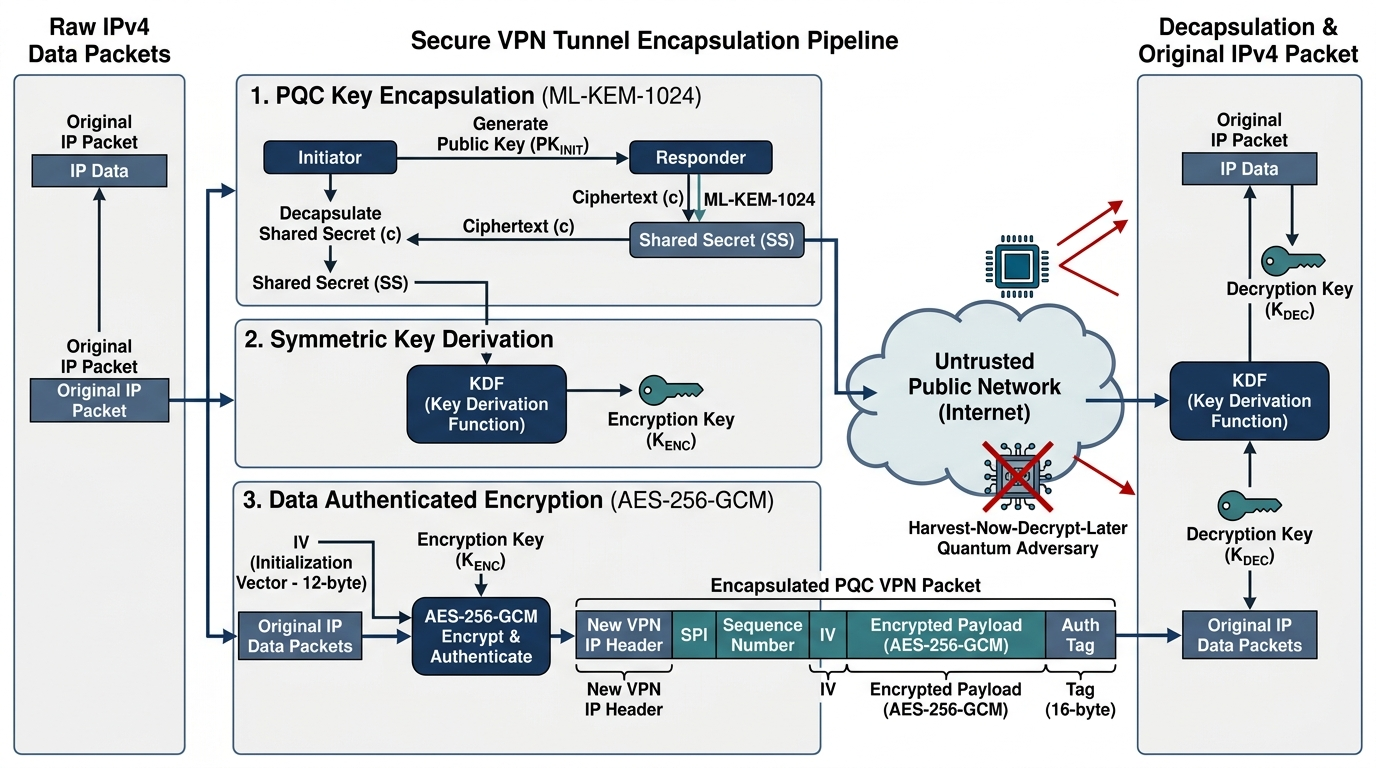
\includegraphics[width=0.92\linewidth,height=0.45\textheight,keepaspectratio]{figures/pqc_tunnel_concept.jpg}
  \caption{Post-Quantum Cryptographic Tunnel Encapsulation Pipeline Combining ML-KEM-1024, HKDF-SHA256, and AES-256-GCM.}
  \label{fig:pqc_tunnel_pipeline}
\end{figure}

\section{Android Operating System VPN Architecture and \texttt{VpnService}}
\label{sec:android_vpn_service_arch}

Android's security architecture enforces process sandboxing, Discretionary Access Control (DAC) via unique Linux User IDs (UIDs) per application, and Mandatory Access Control (MAC) via SELinux policies~\cite{ikram2016measuring}. Under this security model, non-root applications cannot open raw sockets (\texttt{SOCK\_RAW}) or manipulate routing tables directly.

To facilitate legitimate VPN functionality without requiring root privileges, the Android Open Source Project (AOSP) introduced the managed \texttt{android.net.VpnService} framework (API Level~14+)~\cite{android_vpnservice_docs}. The architecture operates as follows:
\begin{enumerate}
    \item \textbf{User Consent and System Dialog}: The application invokes \texttt{VpnService.prepare(context)}. If another VPN is active or permission has not been granted, Android displays a modal system dialog warning the user that the application is requesting permission to intercept all network traffic.
    \item \textbf{Builder Configuration}: Once authorized, the application instantiates a \texttt{VpnService.Builder} instance, configuring:
    \begin{itemize}
        \item \texttt{setSession(String)}: Human-readable session name displayed in the system notification shade.
        \item \texttt{setMtu(int)}: Virtual link MTU (typically 1280--1400 bytes).
        \item \texttt{addAddress(InetAddress, int)}: Virtual IPv4 address and subnet prefix assigned to the mobile TUN adapter (e.g., \texttt{10.8.0.2/24}).
        \item \texttt{addRoute(InetAddress, int)}: Routing prefixes intercepted by the VPN. Setting \texttt{addRoute("0.0.0.0", 0)} establishes a default gateway, capturing all outbound IPv4 traffic.
        \item \texttt{addDnsServer(InetAddress)}: Designated recursive DNS resolvers (e.g., \texttt{1.1.1.1}, \texttt{8.8.8.8}).
    \end{itemize}
    \item \textbf{Interface Establishment}: The builder executes \texttt{establish()}, which instructs the Android Linux kernel to instantiate a virtual TUN interface, configure kernel routing tables, and return a \texttt{ParcelFileDescriptor} (PFD) representing the character device node.
    \item \textbf{Packet I/O}: The application obtains a \texttt{FileInputStream} and \texttt{FileOutputStream} from the PFD. Reading from the input stream yields raw outbound IP packets generated by all running device applications; writing raw IP packets to the output stream injects inbound return packets into the operating system's network stack.
\end{enumerate}

\section{Mobile Network Challenges: Routing Loops and Battery Constraints}
\label{sec:mobile_network_challenges}

Implementing a high-performance VPN client on mobile platforms involves navigating critical operational constraints unique to mobile operating systems.

\subsection{The Routing Loop Dilemma and \texttt{protect()} Mechanism}
When a full-tunnel VPN is established (\texttt{addRoute("0.0.0.0", 0)}), the Linux kernel redirects \textit{all} outgoing IP datagrams into the virtual TUN interface. If the VPN client opens a standard TCP socket to connect to the external VPN server, the kernel intercepts the client's own encrypted VPN frames and routes them back into the TUN interface! This triggers an infinite recursive loop:
\begin{equation}
\text{Packet} \to \text{TUN} \to \text{VPN App} \to \text{Socket} \to \text{Kernel Routing} \to \text{TUN} \to \dots
\end{equation}
This catastrophic feedback loop rapidly exhausts system memory and completely freezes the device's network stack.

To eliminate this loop, the Android framework provides the critical native method \texttt{protect(int socketFd)} (or \texttt{protect(Socket socket)} / \texttt{protect(SocketChannel channel)})~\cite{android_vpnservice_docs}. The \texttt{protect()} system call invokes an underlying \texttt{setsockopt} operation applying the \texttt{SO\_BINDTODEVICE} or \texttt{SO\_MARK} socket option. This explicitly marks the transport socket at the kernel level, commanding the routing subsystem that all traffic originating from this specific file descriptor must bypass the VPN routing table and egress directly through the physical underlying network interface (e.g., \texttt{wlan0} or \texttt{rmnet\_data0}).

\subsection{Mobile Battery and Memory Constraints}
Unlike desktop workstations with continuous AC power and active cooling, mobile smartphones operate under strict energy and thermal budgets. Inefficient user-space VPN implementations that execute frequent allocations, excessive thread context switching, or unoptimized mathematical loops cause severe battery drain and trigger Android's aggressive Low Memory Killer (LMK)~\cite{mavroudis2017touchlog}. A successful mobile post-quantum VPN must minimize memory garbage collection pressure, execute asynchronous non-blocking I/O routines, and leverage hardware-accelerated AES instructions.

\section{Desktop-to-Mobile Application Porting Strategies}
\label{sec:desktop_to_mobile_porting}

Initial post-quantum VPN prototypes developed in academic research are frequently authored in Python on Linux workstations due to the rich ecosystem of experimental cryptography libraries (such as \texttt{liboqs-python}) and rapid prototyping capabilities. However, translating a desktop Python prototype into a native Android application involves addressing significant architectural differences:

\begin{table}[htbp]
  \centering
  \small
  \caption{Architectural Comparison: Desktop Python Prototype vs. Native Android Application.}
  \label{tab:python_vs_android_architecture}
  \begin{tabular}{@{}P{3.5cm}P{5.0cm}P{5.5cm}@{}}
    \toprule
    \textbf{Dimension} & \textbf{Desktop Python Prototype} & \textbf{Native Android Application} \\
    \midrule
    \textbf{Execution Runtime} & CPython 3.12 interpreter & Android Runtime (ART) Ahead-Of-Time (AOT) \\
    \textbf{Language Stack} & Python with C bindings & Kotlin 1.9 with Jetpack Compose (Material 3) \\
    \textbf{TUN Device Access} & Direct Linux \texttt{/dev/net/tun} (Root required) & Sandboxed \texttt{android.net.VpnService} (User consent) \\
    \textbf{Socket Protection} & Manual policy routing / \texttt{ip rule} tables & Native OS \texttt{protect(socket)} bypassing \\
    \textbf{Process Lifecycle} & Persistent CLI daemon & Foreground Service with active Notification \\
    \textbf{Cryptography Engine} & Dynamic C-bindings (\texttt{liboqs}) & Pure-Kotlin lattice arithmetic with SHA-3 alignment \\
    \textbf{State Management} & Global variables and console logging & Reactive MVVM with Kotlin Coroutines \& \texttt{StateFlow} \\
    \textbf{Storage Security} & Plaintext local files & Android Keystore backed \texttt{EncryptedSharedPreferences} \\
    \bottomrule
  \end{tabular}
\end{table}

As detailed in Table~\ref{tab:python_vs_android_architecture}, porting the client requires a complete architectural re-write. The resulting native Kotlin application eliminates interpreter overhead, enforces strict sandboxed permissions, and delivers a robust, consumer-ready graphical interface.

\section{Comparative Survey of Modern VPN Implementations}
\label{sec:comparative_survey}

To position QuantumSafe VPN within the contemporary cybersecurity landscape, Table~\ref{tab:vpn_solutions_matrix} provides a comprehensive comparative analysis of existing commercial and open-source VPN solutions against the proposed implementation across six critical technical dimensions: key exchange mechanism, data encapsulation cipher, quantum resistance status, Android integration framework, wire framing overhead, and open-source auditability.

\begin{table}[htbp]
  \centering
  \footnotesize
  \caption{Comprehensive Technical Comparison of Virtual Private Network Implementations.}
  \label{tab:vpn_solutions_matrix}
  \begin{tabular}{@{}P{2.2cm}P{2.3cm}P{2.2cm}P{2.2cm}P{2.2cm}P{2.6cm}@{}}
    \toprule
    \textbf{Solution} & \textbf{Key Exchange} & \textbf{Data Cipher} & \textbf{Quantum Safe?} & \textbf{Android Integration} & \textbf{Key Limitations} \\
    \midrule
    \textbf{OpenVPN} & TLS (ECDHE / RSA) & AES-256-GCM / CBC & No (Broken by Shor's) & \texttt{VpnService} (OpenVPN Core) & High CPU usage; large C codebase ($>100$k lines) \\
    \addlinespace
    \textbf{WireGuard} & Noise IK (Curve25519) & ChaCha20-Poly1305 & No (Broken by Shor's) & \texttt{VpnService} / Kernel module & Lacks native PQC key exchange \\
    \addlinespace
    \textbf{StrongSwan (IPsec)} & IKEv2 (DH / ECDH) & AES-GCM / AES-CBC & No (Broken by Shor's) & \texttt{VpnService} (IKEv2 client) & Complex configuration; fragile NAT traversal \\
    \addlinespace
    \textbf{Tailscale} & WireGuard (Curve25519) & ChaCha20-Poly1305 & No (Broken by Shor's) & \texttt{VpnService} (Go runtime) & Proprietary coordination server; pre-quantum \\
    \addlinespace
    \textbf{Post-Quantum WireGuard} & Kyber Hybrid in Noise & ChaCha20-Poly1305 & Experimental Hybrid & Experimental (Third-party forks) & Not standardized; non-native mobile packaging \\
    \addlinespace
    \textbf{QuantumSafe VPN (Ours)} & \textbf{ML-KEM-1024 (FIPS 203) + ML-DSA-65} & \textbf{AES-256-GCM (FIPS 197)} & \textbf{Yes (NIST Category 5 Standard)} & \textbf{Native Kotlin VpnService} & TCP-only transport in initial production release \\
    \bottomrule
  \end{tabular}
\end{table}

\section{Summary of Research Gaps and Problem Formulation}
\label{sec:research_gaps}

The rigorous examination of existing literature reveals three distinct research and engineering gaps:
\begin{enumerate}
    \item \textbf{Absence of Standardized PQC in Production Mobile VPNs}: Despite NIST's finalized publication of FIPS 203 and FIPS 204 in August 2024, no mainstream commercial or open-source mobile VPN offers an end-to-end, native Android client implementing pure post-quantum lattice primitives. Existing mobile VPNs remain completely susceptible to Harvest Now, Decrypt Later threats.
    \item \textbf{Cross-Platform Cryptographic Serialization Desynchronization}: Academic post-quantum libraries written in C or Python rely on specific hash implementations (e.g., Keccak SHA-3) that do not always match standard Android JVM cryptographic providers (which default to SHA-2). Bridging this gap requires specialized pure-Kotlin algorithmic implementations that guarantee deterministic cross-platform execution.
    \item \textbf{Usability Deficit in Post-Quantum Security Tools}: Existing post-quantum research prototypes are notoriously difficult to operate, requiring command-line interfaces, manual configuration file editing, and Linux root access. There is an acute lack of user-friendly, accessible mobile user interfaces that convey complex cryptographic telemetry transparently to the end user.
\end{enumerate}

These identified gaps establish the clear mandate for the design, implementation, and evaluation of \textbf{QuantumSafe VPN}.
